\selectlanguage{italian}

\section{Connessioni affini}

Data una varietà differenziabile $ n $-dimensionale $ \mathcal{M} $ ed un campo vettoriale $ \ve{F}(\ve{x}) $ su di essa, fissato un RF $ \{\ve{e}_i (\ve{x})\}_{i = 1, \dots, n} $, nel calcolo della derivata di $ \ve{F}(\ve{x}) $ bisogna considerare anche come varia nello spazio la base:
\begin{equation}
	\frac{\pa \ve{F}}{\pa x^j} = \frac{\pa F^i}{\pa x^j} \ve{e}_i + F^i \frac{\pa \ve{e}^i}{\pa x^j}
	\label{eq:4.1}
\end{equation}
Per trattare formalmente questo problema, è necessario definire la nozione di spazio tangente ad una varietà.
\begin{definition}
	Data una varietà differenziabile $ \mathcal{M} $ ed un suo punto $ p \in \mathcal{M} $, detto $ \mathcal{F}_1(\mathcal{M}) $ lo spazio di tutte le funzioni lisce $ f : I \subseteq \R \rightarrow \mathcal{M} $ (ciascuna determina una curva su $ \mathcal{M} $), si definisce \textit{spazio tangente} a $ \mathcal{M} $ in $ p $ lo spazio:
	\begin{equation}
		T_p\mathcal{M} \defeq \biggl\{ \frac{df}{d\lambda}(\lambda_0) \,\,\forall f \in \mathcal{F}_1(\mathcal{M}) : f(\lambda_0) = p \biggl\}
		\label{eq:4.2}
	\end{equation}
\end{definition}
Sostanzialmente, $ T_p\mathcal{M} $ è lo spazio di tutti i vettori tangenti a $ \mathcal{M} $ spiccati in $ p $.
\begin{definition}
	Data una varietà differenziale $ \mathcal{M} $, fissato un RF $ \{\ve{e}_j(\ve{x})\}_{i = 1, \dots, n} $ su di essa, si definisce la \textit{connessione affine di Levi-Civita} (o \textit{simbolo di Christoffel}) come:
	\begin{equation}
		\Gamma^k_{li} \defeq \ve{e}^k \cdot \frac{\pa \ve{e}_i}{\pa x^l}
		\label{eq:4.3}
	\end{equation}
\end{definition}
Questa connessione affine mette in relazione gli spazi tangenti in due punti a distanza infinitesima.
Riprendendo la derivata di un campo vettoriale:
\begin{equation}
	\ve{e}^k \cdot \frac{\pa \ve{F}}{\pa x^l} = \frac{\pa F^i}{\pa x^l} \underbrace{\ve{e}^k \cdot \ve{e}_i}_{\delta^k_i} + F^i \ve{e}^k \cdot \frac{\pa \ve{e}_i}{\pa x^l} = \frac{\pa F^k}{\pa x^l} + \Gamma^k_{li} F^i \eqdef \nabla_l F^k
	\label{eq:4.4}
\end{equation}
Questa viene definita \textit{derivata covariante} del campo vettoriale $ F^k $ (con abuso di terminologia).
\begin{definition}
	Se $ \Gamma^k_{li} = \Gamma^k_{il} $ si parla di \textit{connessione di Levi-Civita}.
\end{definition}
Ciò vale nelle ipotesi del lemma di Schwarz, poiché $ \ve{e}_i = \frac{\pa \ve{p}}{\pa x^i} $:
\begin{equation}
	\Gamma^k_{li} = \ve{e}^k \cdot \frac{\pa \ve{e}_i}{\pa x^l} = \ve{e}^k \cdot \frac{\pa^2 \ve{p}}{\pa x^l \pa x^i} = \ve{e}^k \cdot \frac{\pa^2 \ve{p}}{\pa x^i \pa x^l} = \ve{e}^k \frac{\pa \ve{e}_l}{\pa x^i} = \Gamma^k_{il}
	\label{eq:4.5}
\end{equation}
Sotto cambio di RF $ x \mapsto y $, la connessione affine trasforma come:
\begin{equation}
	\tilde{\Gamma}^k_{li} = \tilde{\ve{e}}^k \cdot \frac{\pa \tilde{\ve{e}}_i}{\pa y^l} = \frac{\pa y^k}{\pa x^p}\ve{e}^p \frac{\pa x^m}{\pa y^l} \frac{\pa}{\pa x^m} \left( \frac{\pa x^n}{\pa y^i} \ve{e}_n \right) = \frac{\pa y^k}{\pa x^p} \frac{\pa x^m}{\pa y^l} \frac{\pa x^n}{\pa y^i} \Gamma^p_{mn} + \frac{\pa y^k}{\pa x^p} \frac{\pa^2 x^p}{\pa y^l \pa y^i}
	\label{eq:4.6}
\end{equation}
Il secondo termine determina il fatto che, in generale, la connessione affine di Levi-Civita non è un tensore, poiché trasforma in maniera affine, non omogenea.\\
In generale, la connessione affine ha $ n^3 $ componenti indipendenti. Se ci si limita a considerare la connessione di Levi-Civita in nello spaziotempo di Minkowski, essa ha solo 40 componenti indipendenti: per ogni valore $ k = 0,1,2,3 $ ci sono 3 rotazioni, 3 boost e 4 traslazioni.\\
Inoltre, la simmetria $ \Gamma^k_{li} = \Gamma^k_{il} $ è legata a due importanti proprietà:
\begin{itemize}
	\item preservazione della metrica: $ \nabla_l g_{mn} = 0 $;
	\item assenza di torsione nella metrica: $ \left[ X,Y \right] \defeq \nabla_X Y - \nabla_Y X = 0 \,\,\forall X,Y$ campi vettoriali su $ \mathcal{M} $.
\end{itemize}
Sono state definite le parentesi di Lie $ \left[ \cdot,\cdot \right] $.\\
Quando non è presente la suddetta simmetria (es: teoria della gravitazione di Einstein-Cartan), è possibile cancellare il termine non-omogeneo in  Eq. \ref{eq:4.6} definendo un nuovo tensore.
\begin{definition}
	Si definisce il \textit{tensore di torsione} $ T^a_{bc} \defeq \Gamma^a_{bc} - \Gamma^a_{cb} $.
\end{definition}

\section{Trasporto Parallelo}

Data una varietà differenziabile $ n $-dimensionale $ \mathcal{M} $ in un embedding space WLOG identificato con $ \R^{n+k} $, con un opportuno $ k \ge 1 $: è possibile considerare i vettori nei vari $ T_p\mathcal{M} $ come vettori nell'embedding space.\\
Intuitivamente, è possibile immaginare il trasporto parallelo di un vettore lungo una curva sulla varietà come il cambiare punto di applicazione del vettore sull'ipersuperficie nell'embedding space determinata da $ \mathcal{M} $, mantenendo la tangenza alla varietà ma senza modificare le componenti del vettore nell'embedding space. Ciò porta, se si considera una loop sulla varietà, ad ottenere un vettore orientato diversamente da quello iniziale (vedere Fig. \ref{par-tr}).
\begin{figure}
	\centering
	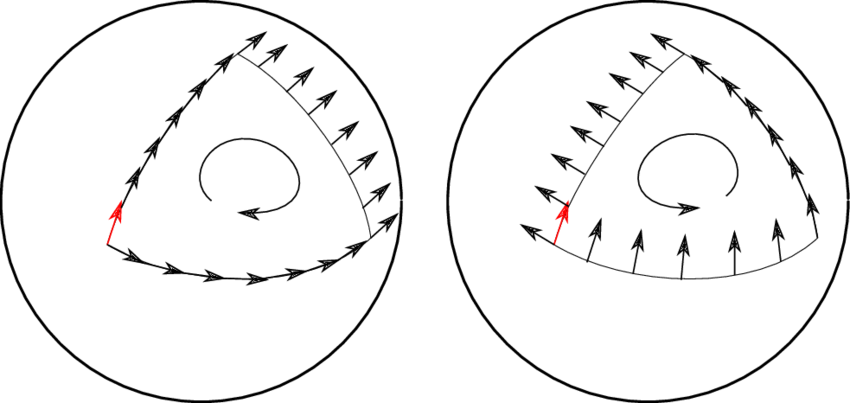
\includegraphics[width=0.60\textwidth]{parallel-transport.png}
	\caption{Parallel transport on a sphere.}
	\label{par-tr}
\end{figure}

\begin{proposition}
	La condizione di trasporto parallello di un campo vettoriale $ \ve{F}(\ve{x}) $ è che lungo la curva considerata si abbia $ \ve{e}^k \cdot d\ve{F} = 0 $.
\end{proposition}
Dato che $ d\ve{F} = \pa_l \ve{F} dx^l $, questa condizione è equivalente a richiedere che $ \nabla_l F^k = 0 $ lungo la curva.

\section{Derivata covariante}

Si introduce la seguente notazione per la derivata: $ f_{,i} = \frac{\pa f}{\pa x^i} $, indipendentemente dalla natura di $ f $.
Considerando un campo vettoriale $ \ve{F}(\ve{x}) $ su una varietà differenziabile $ \mathcal{M} $, quindi, si può riscrivere la derivata covariante come:
\begin{equation}
	\nabla_l F^k \equiv F^k_{;l} \defeq \ve{e}^k \cdot \ve{F}_{,l} = \ve{e}^k \cdot \left( F^i_{,l} \ve{e}_i + F^i \ve{e}_{i,l} \right) = F^k_{,l} + \Gamma^k_{li} F^i
	\label{eq:4.7}
\end{equation}

\begin{proposition}
	$ \ve{e}_k \cdot \ve{e}^i_{,l} = - \Gamma^i_{lk} $.
\end{proposition}
\begin{proof}
	$ 0 = \delta^i_{k,l} = \left( \ve{e}_k \cdot \ve{e}^i \right)_{,l} = \ve{e}_{k,l} \cdot \ve{e}^i + \ve{e}_k \cdot \ve{e}^i_{,l} = \Gamma^i_{lk} + \ve{e}_k \cdot \ve{e}^i_{,l} $.
\end{proof}
È dunque possibile esprimere la derivata covariante sia di un campo controvariante che di un campo covariante:
\begin{equation}
	V^k_{;l} \defeq \ve{e}^k \cdot \ve{V}_{,l} = \ve{e}^k \cdot \left( V^i_{,l} \ve{e}_i + V^i \ve{e}_{i,l} \right)
	\label{eq:4.8}
\end{equation}
\begin{equation}
	V_{k;l} \defeq \ve{e}_k \cdot \ve{V}_{,l} = \ve{e}_k \cdot \left( V_{i,l} \ve{e}^i + V_i \ve{e}^i_{,l} \right)
	\label{eq:4.9}
\end{equation}
Scrivendo in funzione delle connessioni affini:
\begin{equation}
	\nabla_l V^k = \frac{\pa V^k}{\pa x^l} + \Gamma^k_{li} V^i
	\label{eq:4.10}
\end{equation}
\begin{equation}
	\nabla_l V_k = \frac{\pa V_k}{\pa x^l} - \Gamma^i_{lk} V_i
	\label{eq:4.11}
\end{equation}
Sulle varietà torsion-free ($ T^a_{bc} \equiv 0 $) si può definire il rotore covariante come $ V_{l;i} - V_{i;l} = V_{l,i} - V_{i,l} $.

\begin{proposition}
	La derivata covariante trasforma come un tensore.
\end{proposition}
\begin{proof}
	Ricordando Eq. \ref{eq:4.6}:
	\begin{equation*}
		\begin{split}
			\tilde{\nabla}_l \tilde{V}^k
			&= \frac{\pa \tilde{V}^k}{\pa y^l} + \tilde{\Gamma}^k_{li}\tilde{V}^i = \frac{\pa x^m}{\pa y^l} \frac{\pa}{\pa x^m} \left( \frac{\pa y^k}{\pa x^p} V^p \right) + \tilde{\Gamma}^k_{lj} \tilde{V}^j\\
			&= \frac{\pa x^m}{\pa y^l} \frac{\pa y^k}{\pa x^p} \frac{\pa V^p}{\pa x^m} + \frac{\pa x^m}{\pa y^l} \frac{\pa^2 y^k}{\pa x^m \pa x^n} V^n + \frac{\pa y^k}{\pa x^p} \frac{\pa x^m}{\pa y^l} \underbrace{\frac{\pa x^n}{\pa y^j} \frac{\pa y^j}{\pa x_i}}_{\delta^n_i} \Gamma^p_{mn} V^i + \frac{\pa y^k}{\pa x^p} \frac{\pa^2 x^p}{\pa y^l \pa y^j} \frac{\pa y^j}{\pa x^n} V^n\\
			&= \frac{\pa x^m}{\pa y^l} \frac{\pa y^k}{\pa x^p} \left( \frac{\pa V^p}{\pa x^m} + \Gamma^p_{mn} V^n \right) + \left( \frac{\pa x^m}{\pa y^l} \frac{\pa^2 y^k}{\pa x^m \pa x^n} + \frac{\pa y^k}{\pa x^p} \frac{\pa^2 x^p}{\pa y^l \pa y^j} \frac{\pa y^j}{\pa x^n} \right) V^n
		\end{split}
	\end{equation*}
	Basta mostrare che il secondo termine è nullo:
	\begin{equation*}
		\begin{split}
			\frac{\pa}{\pa y^l} \frac{\pa y^k}{\pa x^n} + \frac{\pa y^k}{\pa x^p} \left[ \frac{\pa y^j}{\pa x^n} \frac{\pa}{\pa y^l} \frac{\pa x^p}{\pa y^j} \right]
			&= \frac{\pa}{\pa y^l} \frac{\pa y^k}{\pa x^n} + \frac{\pa y^k}{\pa x^p} \left[ \frac{\pa}{\pa y^l} \left( \frac{\pa y^j}{\pa x^n} \frac{\pa x^p}{\pa y^j} \right) - \frac{\pa x^p}{\pa y^j} \frac{\pa}{\pa y^l} \frac{\pa y^j}{\pa x^n} \right]\\
			&= \frac{\pa}{\pa y^l} \frac{\pa y^k}{\pa x^n} + \frac{\pa y^k}{\pa x^p} \left( \frac{\pa}{\pa y^l} \delta^p_n \right) - \delta^k_j \frac{\pa}{\pa y^l} \frac{\pa y^j}{\pa x^n} = \frac{\pa}{\pa y^l} \frac{\pa y^k}{\pa x^n} - \frac{\pa}{\pa y^l} \frac{\pa y^k}{\pa x^n} = 0
		\end{split}
	\end{equation*}
	Il caso della derivata covariante di un vettore covariante è analogo.
\end{proof}

\begin{proposition}\label{cov-2}
	La derivata covariante di un tensore di rango 2 è:
	\begin{equation}
		\nabla_k A_{ij} = \frac{\pa A_{ij}}{\pa x^k} - \Gamma^m_{ik} A_{mj} - \Gamma^m_{jk} A_{im}
		\label{eq:4.12}
	\end{equation}
	\begin{equation}
		\nabla_k A^{ij} = \frac{\pa A^{ij}}{\pa x^k} + \Gamma^i_{mk} A^{mj} + \Gamma^j_{mk} A^{im}
		\label{eq:4.13}
	\end{equation}
\end{proposition}
\begin{proof}
	$ \tens{A} = A_{ij} \ve{e}^i \otimes \ve{e}^j $, quindi:
	\begin{equation*}
		\begin{split}
			\frac{\pa \tens{A}}{\pa x^k}
			&= \frac{\pa A_{ij}}{\pa x^k} \ve{e}^i \otimes \ve{e}^j + A_{ij} \frac{\pa\ve{e}^i}{\pa x^k} \otimes \ve{e}^j + A_{ij} \ve{e}^i \otimes \frac{\pa\ve{e}^j}{\pa x^k}\\
			&= \frac{\pa A_{ij}}{\pa x^k} \ve{e}^i \otimes \ve{e}^j - A_{ij} \Gamma^i_{mk} \ve{e}^m \otimes \ve{e}^j - A_{ij} \Gamma^j_{mk} \ve{e}^i \otimes \ve{e}^m\\
			&= \frac{\pa A_{ij}}{\pa x^k} \ve{e}^i \otimes \ve{e}^j - A_{mj} \Gamma^m_{ik} \ve{e}^i \otimes \ve{e}^j - A_{im} \Gamma^m_{jk} \ve{e}^i \otimes \ve{e}^j\\
			&= \left( \frac{\pa A_{ij}}{\pa x^k} - \Gamma^m_{ik} A_{mj} - \Gamma^m_{jk} A_{im} \right) \ve{e}^i \otimes \ve{e}^j \eqdef \left( \nabla_k A_{ij} \right) \ve{e}^i \otimes \ve{e}^j
		\end{split}
	\end{equation*}
\end{proof}

\begin{proposition}
	Dato $ A_{ij} $ tensore di rango 2 antisimmetrico su una varietà torsion-free, si ha:
	\begin{equation}
		A_{ij;k} + A_{ki;j} + A_{jk;i} = A_{ij,k} + A_{ki,j} + A_{jk,i}
		\label{eq:4.14}
	\end{equation}
\end{proposition}
\begin{proof}
	Dalla Prop. \ref{cov-2}:
	\begin{equation*}
		\begin{split}
			A_{ij;k} + A_{ki;j} + A_{jk;i}
			&= A_{ij,k} - \Gamma^m_{ik} A_{mj} - \Gamma^m_{jk} A_{im} + A_{ki,j} - \Gamma^m_{kj} A_{mi} - \Gamma^m_{ij} A_{km} \\ &\qquad \qquad \qquad \qquad \qquad \qquad \qquad \qquad + A_{jk,i} - \Gamma^m_{ji} A_{mk} - \Gamma^m_{ki} A_{jm}
		\end{split}
	\end{equation*}
	Per simmetria di $ \Gamma^m_{ik} $ ed antisimmetria di $ A_{ij} $:
	\begin{equation*}
		\Gamma^m_{ik} A_{mj} = - \Gamma^m_{ki} A_{jk} \qquad \Gamma^m_{jk} A_{im} = - \Gamma^m_{kj} A_{mi} \qquad \Gamma^m_{ij} A_{km} = - \Gamma^m_{ji} A_{mk}
	\end{equation*}
	da cui segue la tesi.
\end{proof}

Ciò dimostra che l'identità di Bianchi è valida in qualsiasi sistema di riferimento su una varietà torsion-free.










